\section{Vorbereitung}
Damit das Projekt erfolgreich umgesetzt werden kann, sind im Vorfeld mehrere technische und organisatorische Vorbereitungen erforderlich. 
Insbesondere die Einrichtung der ROS-2-Umgebung sowie die Sicherstellung einer stabilen Netzwerkverbindung zwischen dem Steuerrechner und dem TurtleBot3 stellen grundlegende Voraussetzungen für die Durchführung des Projekts dar. 
Darüber hinaus wird eine erste praktische Auseinandersetzung mit ROS 2 vorgenommen, um ein grundlegendes Verständnis der Funktionsweise und Struktur des Systems zu erlangen.
\subsection{Installation ROS 2}
Zur Herstellung einer funktionalen Kommunikationsverbindung zwischen dem Steuerrechner und dem TurtleBot3 wurde der offizielle Quick Start Guide \cite{tb3_quickstart} von Robotis herangezogen. 
Um die Kompatibilität beider Systeme sicherzustellen, wurde auf dem Rechner dieselbe Version von ROS 2 (Humble Hawksbill) installiert.
Dazu wurde zunächst eine virtuelle Maschine mit Ubuntu 22.04 eingerichtet. 
Anschließend erfolgte die Installation aller für ROS 2 relevanten Pakete sowie der Standardsoftware für den TurtleBot3, darunter Tools zur Kartografierung, Sen\-sor\-da\-ten\-er\-fass\-ung und Robotersteuerung.
\newPar
Um eine konsistente Kommunikation zu ermöglichen, wurden auf beiden Systemen spezifische Parameter vereinheitlicht: Als Modell wurde \textit{BURGER} gewählt, welches der Hardwarekonfiguration des eingesetzten TurtleBot3 entspricht. Die Domain-ID für ROS 2 wurde auf den Wert \textit{5} gesetzt, um die Kommunikation auf eine definierte Gruppe von ROS-Nodes zu beschränken. 
Zudem kam mit \textit{rmw\_fastrtps\_cpp} eine Middleware-Implementierung zum Einsatz, die auf dem DDS-Standard basiert und für die Datenübertragung zwischen ROS-2-Nodes zuständig ist.
\newPar
Darüber hinaus wurde die ROS-Installation auf dem TurtleBot vollständig neu durchgeführt, um potenzielle Konflikte mit vorherigen Installationen oder Konfigurationen auszuschließen.
\subsection{Netzwerkverbindung}
Für die bidirektionale Kommunikation zwischen dem TurtleBot3 und dem Steuerrechner war die Einbindung beider Geräte in ein gemeinsames Netzwerk erforderlich. 
In der Anfangsphase des Projekts wurde hierzu ein Smartphone-Hotspot verwendet. 
Dieser Ansatz erwies sich jedoch aufgrund erheblicher Schwankungen in der Übertragungsqualität als unzuverlässig.
\newPar
Im weiteren Verlauf wurde daher ein WLAN-Repeater eingesetzt, der ein stabiles und gemeinsames Netzwerk für beide Geräte bereitstellte. 
Zur Einbindung der Geräte in dieses Netzwerk wurden entsprechende Anpassungen an der Netzwerkkonfiguration des Turtlebots in der Datei \textit{/etc/netplan/50-cloud-init.yaml} vorgenommen und durch den Befehl \textit{sudo netplan apply} aktiviert.
Durch diese optimierte Lösung konnte eine stabile Datenübertragung sichergestellt werden, insbesondere für die Übermittlung der Bilddaten in Echtzeit.
\newPar
Sobald beide Systeme erfolgreich im Netzwerk verbunden waren, wurde die Kommunikation über das SSH-Protokoll eingerichtet. 
Dies ermöglichte den Fernzugriff auf den TurtleBot3 ohne zusätzliche Peripheriegeräte wie Bildschirm oder Tastatur, was die Handhabung im Projektalltag deutlich vereinfacht hat.
\subsection{Einarbeitung ROS 2}
Zur Überprüfung der erfolgreichen Systeminstallation wurde das vorinstallierte Teleop-Programm genutzt, mit dem sich der TurtleBot3 manuell über die Tastatur steuern lässt. 
Darüber hinaus wurde mithilfe von rqt ein erster Einblick in die Kommunikation über Topics gewonnen. 
Der Topic Monitor (\imageref{rqt}) erlaubte die Analyse von Sensordatenströmen und bot eine visuelle Darstellung aktiver Kommunikationskanäle.
\begin{figure}[H]
    \centering
    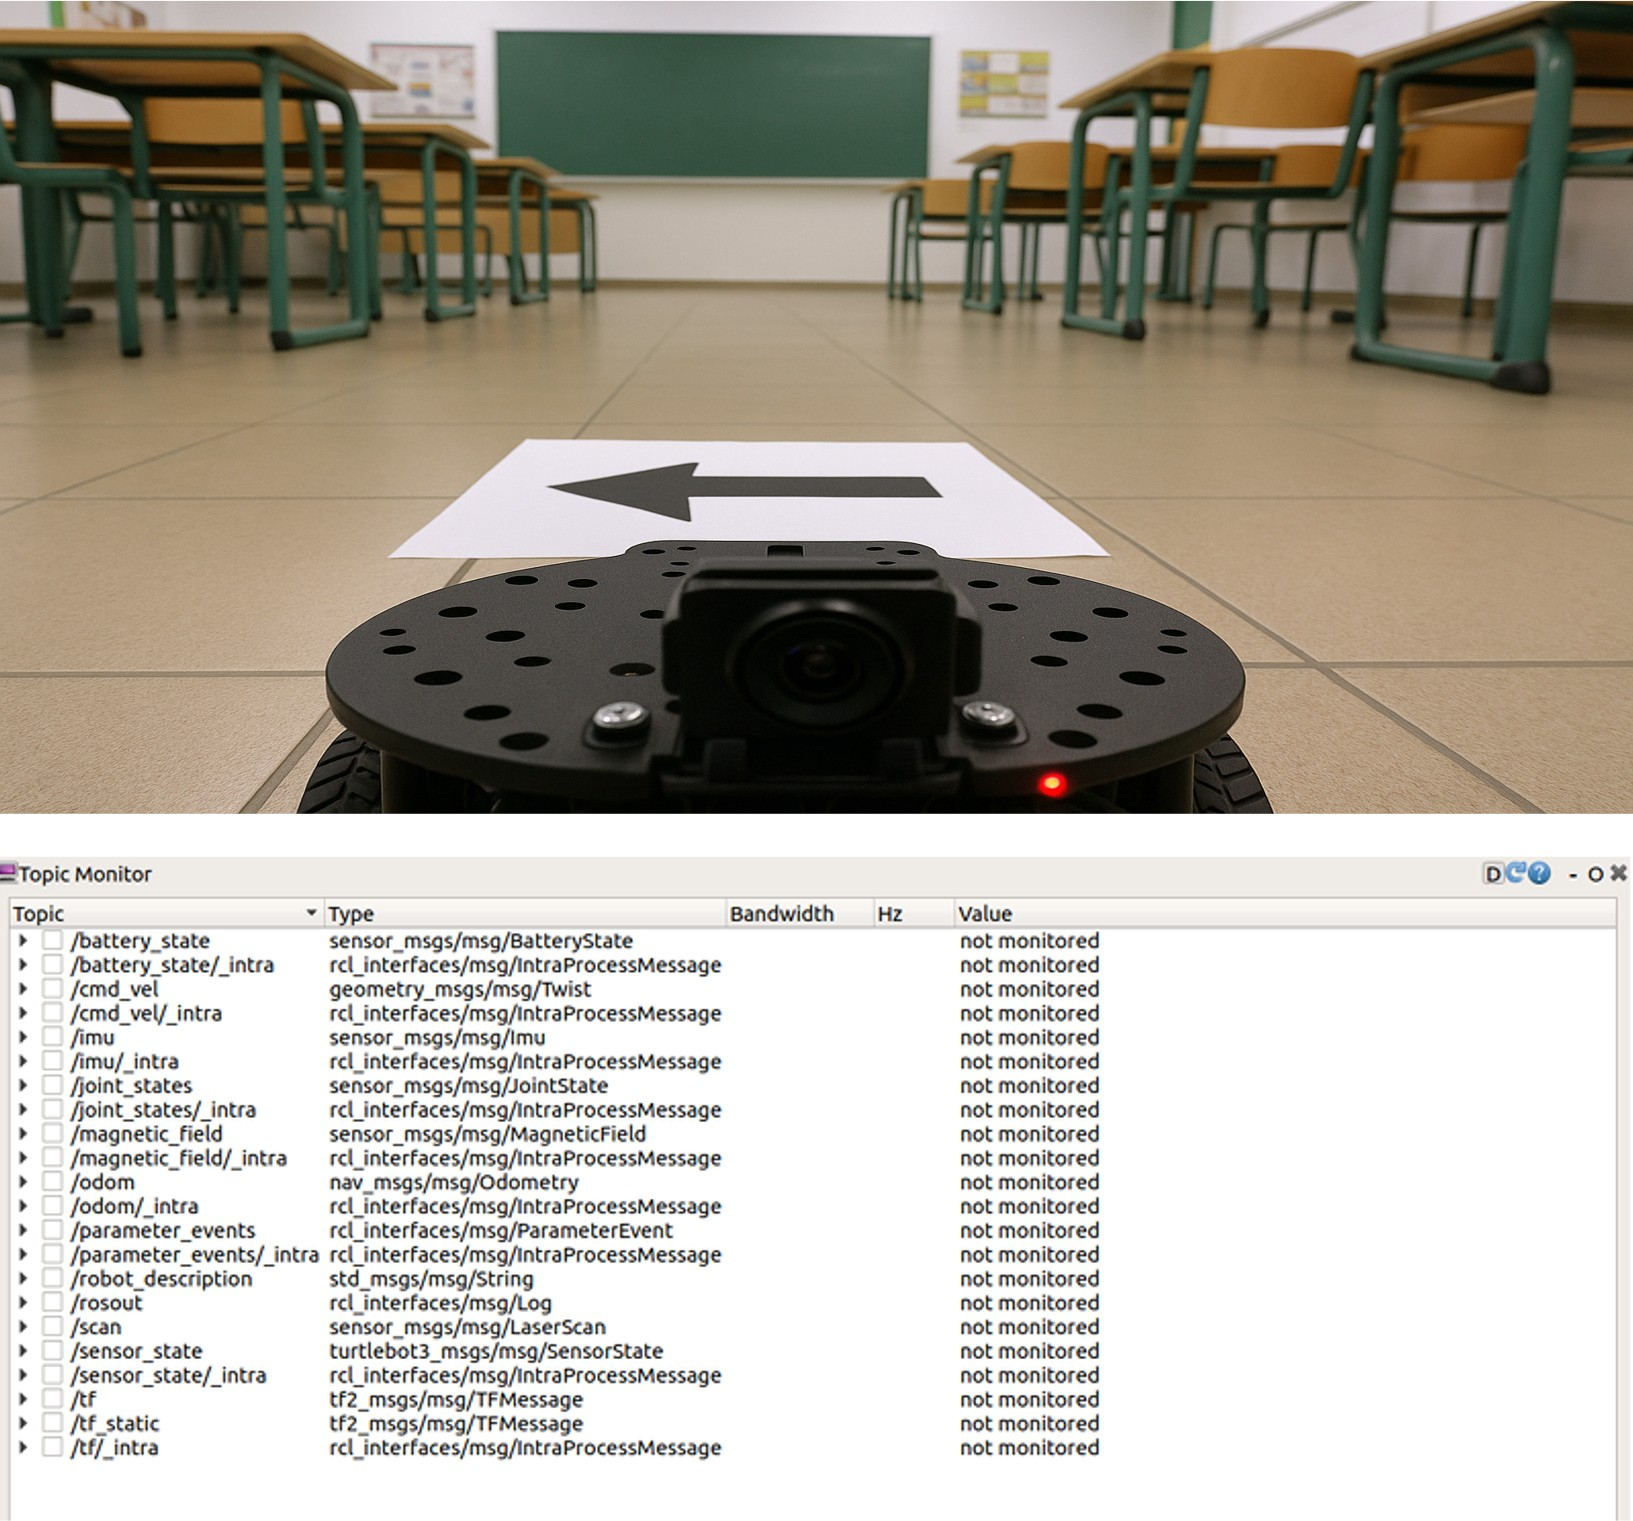
\includegraphics[width=\linewidth]{rqt}
    \caption{Topic-Monitor mit Image-View-Plugin (RQT)}\label{rqt}
\end{figure}
Im Rahmen der weiteren Einarbeitung wurde zudem die SLAM-Funktionalität (Simultaneous Localization and Mapping) getestet, um ein besseres Verständnis für die Navigation und Kartenerstellung mit dem TurtleBot3 in Kombination mit ROS 2 zu gewinnen. 
Diese ersten praktischen Erfahrungen bildeten die Grundlage für die darauf aufbauenden Entwicklungen im weiteren Projektverlauf.
\subsection{Einbinden der Kamera}
Der TurtleBot3 besitzt in seiner Standardausführung keine integrierte Kamera. 
Zu Beginn des Projekts war allerdings bereits eine externe Raspberry Pi Camera 1.3 nachgerüstet. 
Um diese korrekt in das System zu integrieren und mit ROS 2 nutzbar zu machen, waren mehrere Konfigurations- und Installationsschritte notwendig.
\newPar
Zunächst wurden auf dem Raspberry Pi alle erforderlichen Systempakete installiert, darunter \textit{libraspberrypi-bin}, \textit{v4l-utils} sowie das ROS-2-Paket \textit{ros-humble-v4l2-camera}, das die Nutzung von Kameras über das Video4Linux2-Interface ermöglicht. 
Zusätzlich wurde das Paket \textit{ros-humble-image-transport-plugins} installiert, um verschiedene Bildübertragungsformate (\zB~komprimierte Streams) in ROS~2 nutzen zu können. 
Damit der Benutzer auf die Kamera zugreifen darf, wurde dieser der Benutzergruppe \textit{video} hinzugefügt.
\newPar
Anschließend erfolgte die Konfiguration der Kamera über das Tool \textit{raspi-config}. 
Hierbei wurden im Menü unter \textit{Interface Options} sowohl die Legacy\hyp{}Kameraunterstützung als auch SPI und I2C aktiviert. 
Nach einem Systemneustart wurde mit dem Befehl \textit{vcgencmd get\_camera} überprüft, ob die Kamera korrekt erkannt wurde.
\newPar
Zum Start der Kamera in ROS 2 wurde schließlich der Node \textit{v4l2\_camera\_node} ausgeführt, wobei die gewünschte Auflösung von 640x480 Pixeln als Parameter übergeben wurde. 
Diese moderate Auflösung wurde gewählt, um ein flüssiges Videobild bei gleichzeitig geringer Systemauslastung sicherzustellen.
\subsection{Zusammenarbeit über Git}
Um im späteren Verlauf des Projekts eine parallele Entwicklung des Codes zu ermöglichen und einen einfachen Austausch zwischen den verwendeten Systemen sicherzustellen, wurde Git als Versionsverwaltungssystem eingesetzt. 
Zu diesem Zweck wurde ein zentrales Git-Repository eingerichtet, das der Projektgruppe eine strukturierte und nachvollziehbare Zusammenarbeit ermöglichte.
\newPar
Das Repository wurde in mehrere Branches unterteilt, um unterschiedliche Aufgabenbereiche klar zu trennen: 
Ein Branch diente der Projektdokumentation, ein weiterer dem späteren Training des YOLO-Modells, und ein dritter Branch wurde für die Implementierung der ROS 2-Nodes vorbereitet. 
Diese Aufteilung erleichterte nicht nur die Zusammenarbeit, sondern stellte auch sicher, dass Änderungen gezielt getestet und unabhängig voneinander weiterentwickelt werden konnten.